\documentclass{osa-article}

%% Select the journal you're submitting to
%% oe, boe, ome, osac, osajournal
\journal{oe}
% Key:
% Express journals must have the correct journal selected:
% {oe} Optics Express
% {boe} Biomedical Optics Express
% {ome} Optical Material Express
% {optcon} Optics Continuum
% Other OSA journals may use:
% {osajournal} Applied Optics, Advances in Optics and Photonics, Journal of the Optical Society of America A/B, Optics Letters, Optica, Photonics Research

% Uncomment if submitting to Photonics Research.
% ONLY APPLICABLE FOR \journal{osajournal}
% \setprjcopyright

% Set the article type
%\articletype{Research Article}
% Note that article type is not required for Express journals (OE, BOE, OME and OSAC)
% \usepackage[hang,small,bf]{caption}
\usepackage[subrefformat=parens]{subcaption}
\captionsetup{compatibility=false}
\usepackage{todonotes}
\usepackage{lineno}
\usepackage{layout}
\usepackage{lipsum}
\usepackage{bm, amsmath, comment, color, soul, cite, siunitx}
\sisetup{parse-numbers = false}
\linenumbers

\begin{document}

\title{Universal manuscript template for Optica Publishing Group journals}

\author{Yasutaka IMAI,\authormark{1, *}, Hidetoshi HARA,\authormark{1, *}}

\address{\authormark{1}Reserch Institute for Interdisciplinary Science, Okayama University, Okayama, Japan}

\email{\authormark{*}imai1117@okayama-u.ac.jp} %% email address is required

% \homepage{http:...} %% author's URL, if desired

%%%%%%%%%%%%%%%%%%% abstract %%%%%%%%%%%%%%%%
%% [use \begin{abstract*}...\end{abstract*} if exempt from copyright]
\begin{comment}
  The abstract should be limited to approximately 100 words
  If the work of another author is cited in the abstract, that citation should be written out without a number, (e.g., journal, volume, first page, and year in square brackets [Opt. Express {\bfseries 22}, 1234 (2014)]), and a separate citation should be included in the body of the text
  The first reference cited in the main text must be [1]
  Do not include numbers, bullets, or lists inside the abstract.
\end{comment}
\begin{abstract}
We reported on a single stage \SI{976}{nm} Yb-doped fiber amplifier(YDFA) and a double stage \SI{1112}{nm} YDFA with commercially available Yb-doped fibers.
In developing of two YDFAs of different wavelengths, we estimated upper limit of Yb-doped fiber length and output of signal and ASE by numerical simulation.
The simulataion results showed good agreement with experimental results, and both YDFAs achieved stable several Watts continuous-wave(CW) outputs.
\end{abstract}

%%%%%%%%%%%%%%%%%%%%%%%%%%  body  %%%%%%%%%%%%%%%%%%%%%%%%%%
\listoftodos
\section{Introduction}
Rare-earth-doped fiber laser and amplifier systems are useful in a various fields.
For example, the high-power and compact systems are used in laser processing, long-distance optical communication, and LiDAR systems.
In physics, highly stable doped fiber systems are attracting as a light source for experiment \cite{burkleyYbFiberAmplifier2017, coluccelliOpticalFrequencyComb2016}.
Although there are still some problems which are not fully understood such as photodarkening \cite{paschottaLifetimeQuenchingYbdoped1997}, remarkable progress has been made in their performance.

Single-frequency light sources at \SI{976}{nm} and \SI{1112}{nm} also such as spectroscopy of Yb atoms \todo{uncomplete sentence} \cite{franzenSinglestage1112Nm2018}.
However, they are difficult to design because \SI{976}{nm} is in the middle of the absorption band and \SI{1112}{nm} is at the edge of the emission band of Yb-doped fiber.
Therefore, numeraical simulation is indispensable.

\section{Experimental setup}
\subsection{976\,nm amplifier system}

\begin{figure}[h!]
  \centering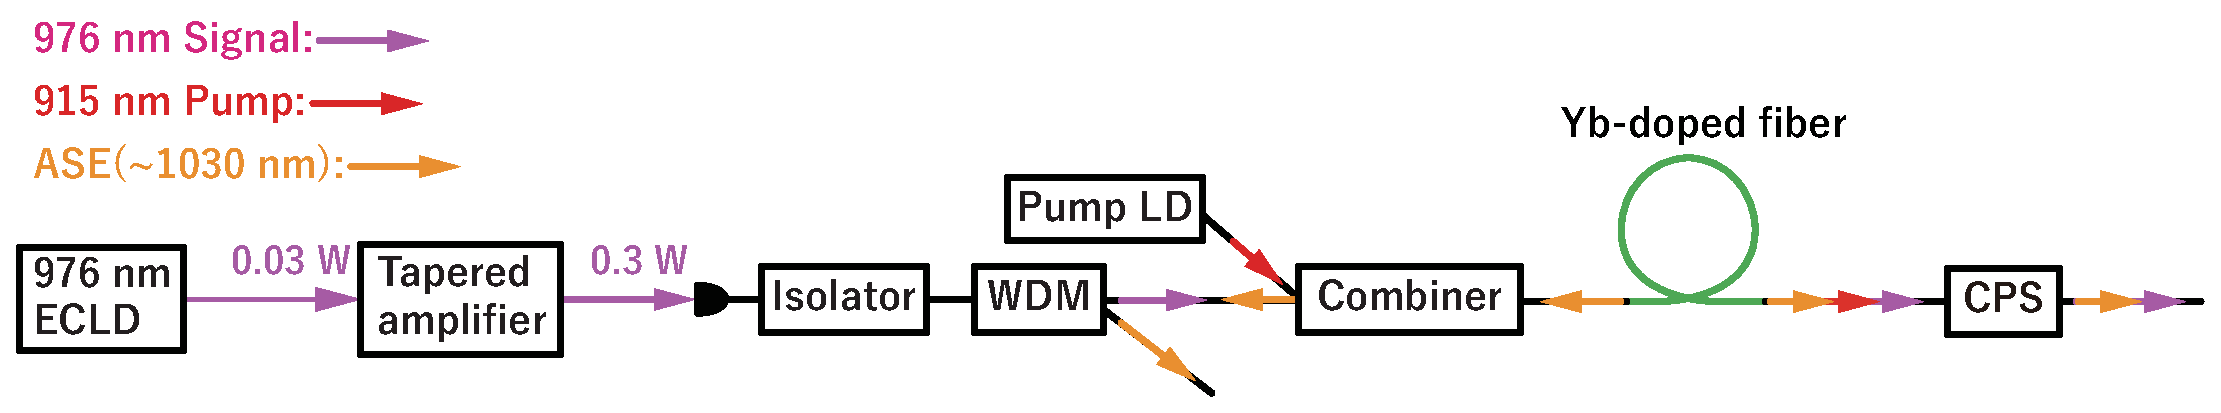
\includegraphics[width=\linewidth]{./Figure/976nmYDFASystem.eps}
  \caption{\SI{976}{\nm} YDFA system.}
  \label{fig:976YDFASystem}
\end{figure}

A schematic of the \SI{976}{\nm} YDFA system is shown in Fig.~\ref{fig:976YDFASystem}.
An external-cavity laser diode(ECLD) at \SI{976}{\nm} is used for the seed laser.
The seed laser is pre-amplified by tapered amplifier from \SI{30}{\mW} to \SI{900}{\mW}, and coupled to the YDFA input fiber which is a polarization maintining(PM) fiber with a FPC/AC connector.
The seed input of the YDFA is connected to an isolator and a wavelength division multiplexing(WDM) filter, which are used to block return light to the seed laser such as backward ASE.
The seed and pump are combined into a double cladding PM fiber, which has a core diameter of \SI{20}{\um} and a cladding diameter of \SI{125}{\um} by a pump and signal combiner.
The \SI{915}{\nm} radiation for pumping the Yb-doped fiber is generated from fiber-coupled laser diode with an output power of up to \SI{70}{\W}.
The combiner output is spliced to the Yb-doped fiber.
The Yb-doped fiber nLIGHT Yb1200-25/125DC-PM is used as the gain fiber.
The fiber is fixed on top of the water-cooled heatsink with a thermal conductive sheet.
The cladding power stripper(CPS) is connected after Yb-doped fiber to remove a residual pump power in the output of Yb-doped fiber.
The output of YDFA system collimated by pigtailed collimator is separated into the ASE around 1030 nm and other wavelengths by a filter.

\begin{comment}
\subsection{987\,nm amplifier system}

\begin{figure}[h!]
  \centering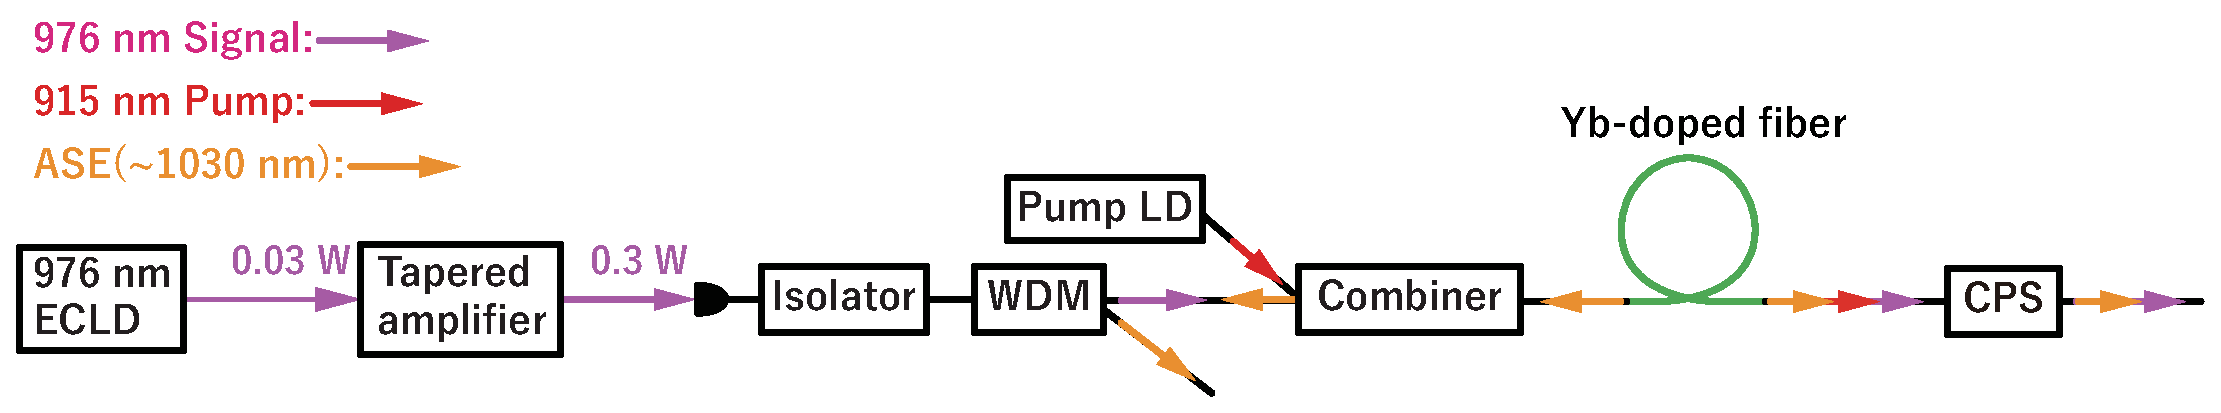
\includegraphics[width=\linewidth]{./Figure/976nmYDFASystem.eps}
  \caption{\SI{987}{\nm} YDFA system.}
  \label{fig:987YDFASystem}
\end{figure}

The design of the \SI{987}{\nm} YDFA system is shown in Fig.~\ref{fig:987YDFASystem}.
The \SI{987}{\nm} YDFA has almost the same configuration as the \SI{976}{\nm} YDFA system.
The seed laser is composed of ECLD at \SI{987}{\nm}.
The maximum seed and pump powers after a combiner are \SI{30}{\mW} and \SI{30}{\W}, respectively.
\end{comment}


\subsection{1112\,nm amplifier system}

\begin{figure}[h!]
  \centering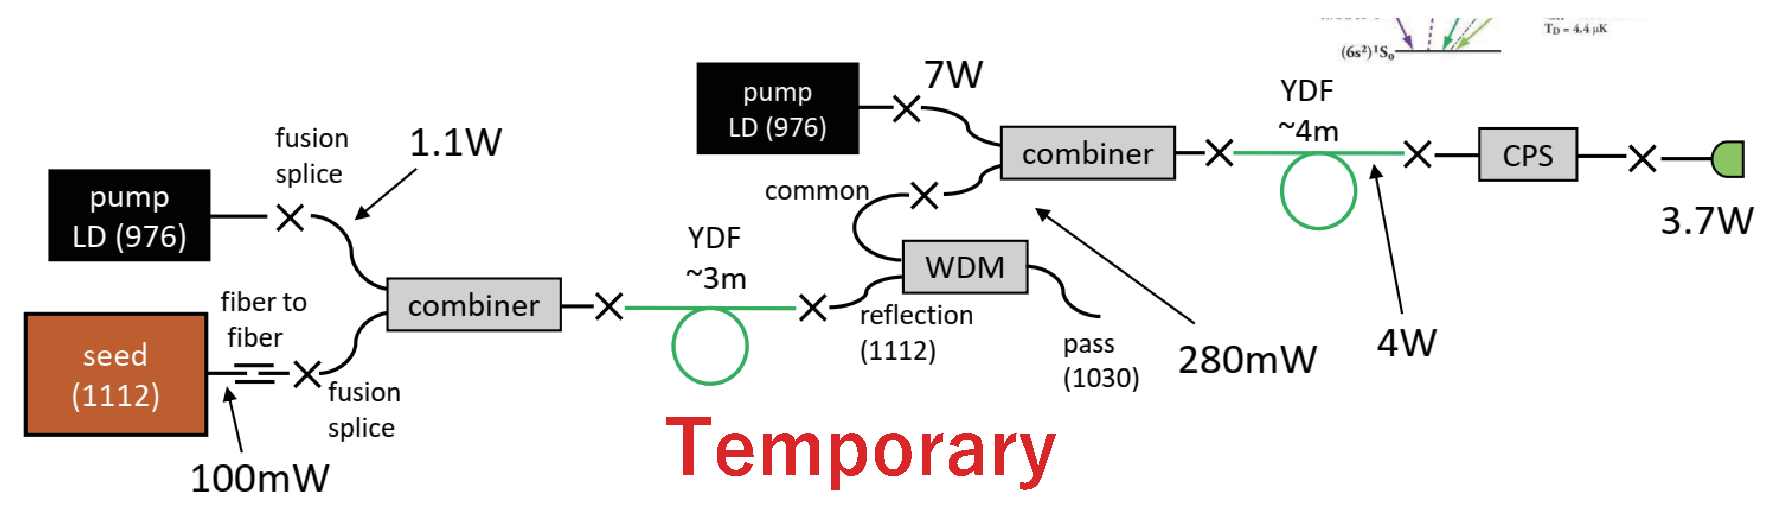
\includegraphics[width=\linewidth]{./Figure/1112nmYDFASystem_Temp.eps}
  \caption{\SI{1112}{\nm} YDFA system.}
  \label{fig:1112YDFASystem}
\end{figure}

The configuration of the \SI{1112}{\nm} YDFA system is shown in Fig.~\ref{fig:1112YDFASystem}.
The \SI{1112}{\nm} YDFA system consists of a two-stage amplifier.
The fiber laser at \SI{1112}{\nm}(Menlo systems Orange one-2) is used as the seed laser.
% The seed output fiber with a FPC/AC connector is contacted to the input fiber of the first amplifier stage with a mating sleeve.
In the first stage, the seed laser and the pump laser, which is generated by fiber-coupled laser diode at \SI{976}{\nm} with a maximum output of \SI{7}{\W}, are mixed with the first combiner.
The first combiner has a signal port, two pump ports, and a common port, which are a single-mode fiber of \SI{5.8/125}{\um}, multi-mode fibers of \SI{105/125}{\um}, and a double-cladding fiber \SI{10/125}{\um}.
The seed power at the common port of the first combiner is \SI{80?}{\mW}.
The Yb-doped fiber(nLIGHT Yb1200-10/125DC) is used as a gain fiber.
The length of the Yb-doped fiber is about \SI{1?}{m}.
The output from Yb-doped fiber is separated into \SI{1112}{\nm} signal component and ASE component around \SI{1030}{\nm} by WDM, and only the \SI{1112}{\nm} signal component is coupled to the the second amplifier stage.
The second Yb-doped fiber is the same one of the first Yb-doped fiber.
The about \SI{3?}{m} long doped fiber is coiled to a diameter of \SI{10}{\cm} and fixed inside an aluminum enclosure with thermal conductive sheet.
Temperature of the aluminum enclosure is controlled by peltier devices.
Output of the second Yb-doped fiber is removed by CPS and collimated by pigtailed collimator.


\section{Results and discussion}
\subsection{976\,nm YDFA}

\begin{figure}[h!]
  \begin{minipage}[b]{0.5\linewidth}
    \centering
    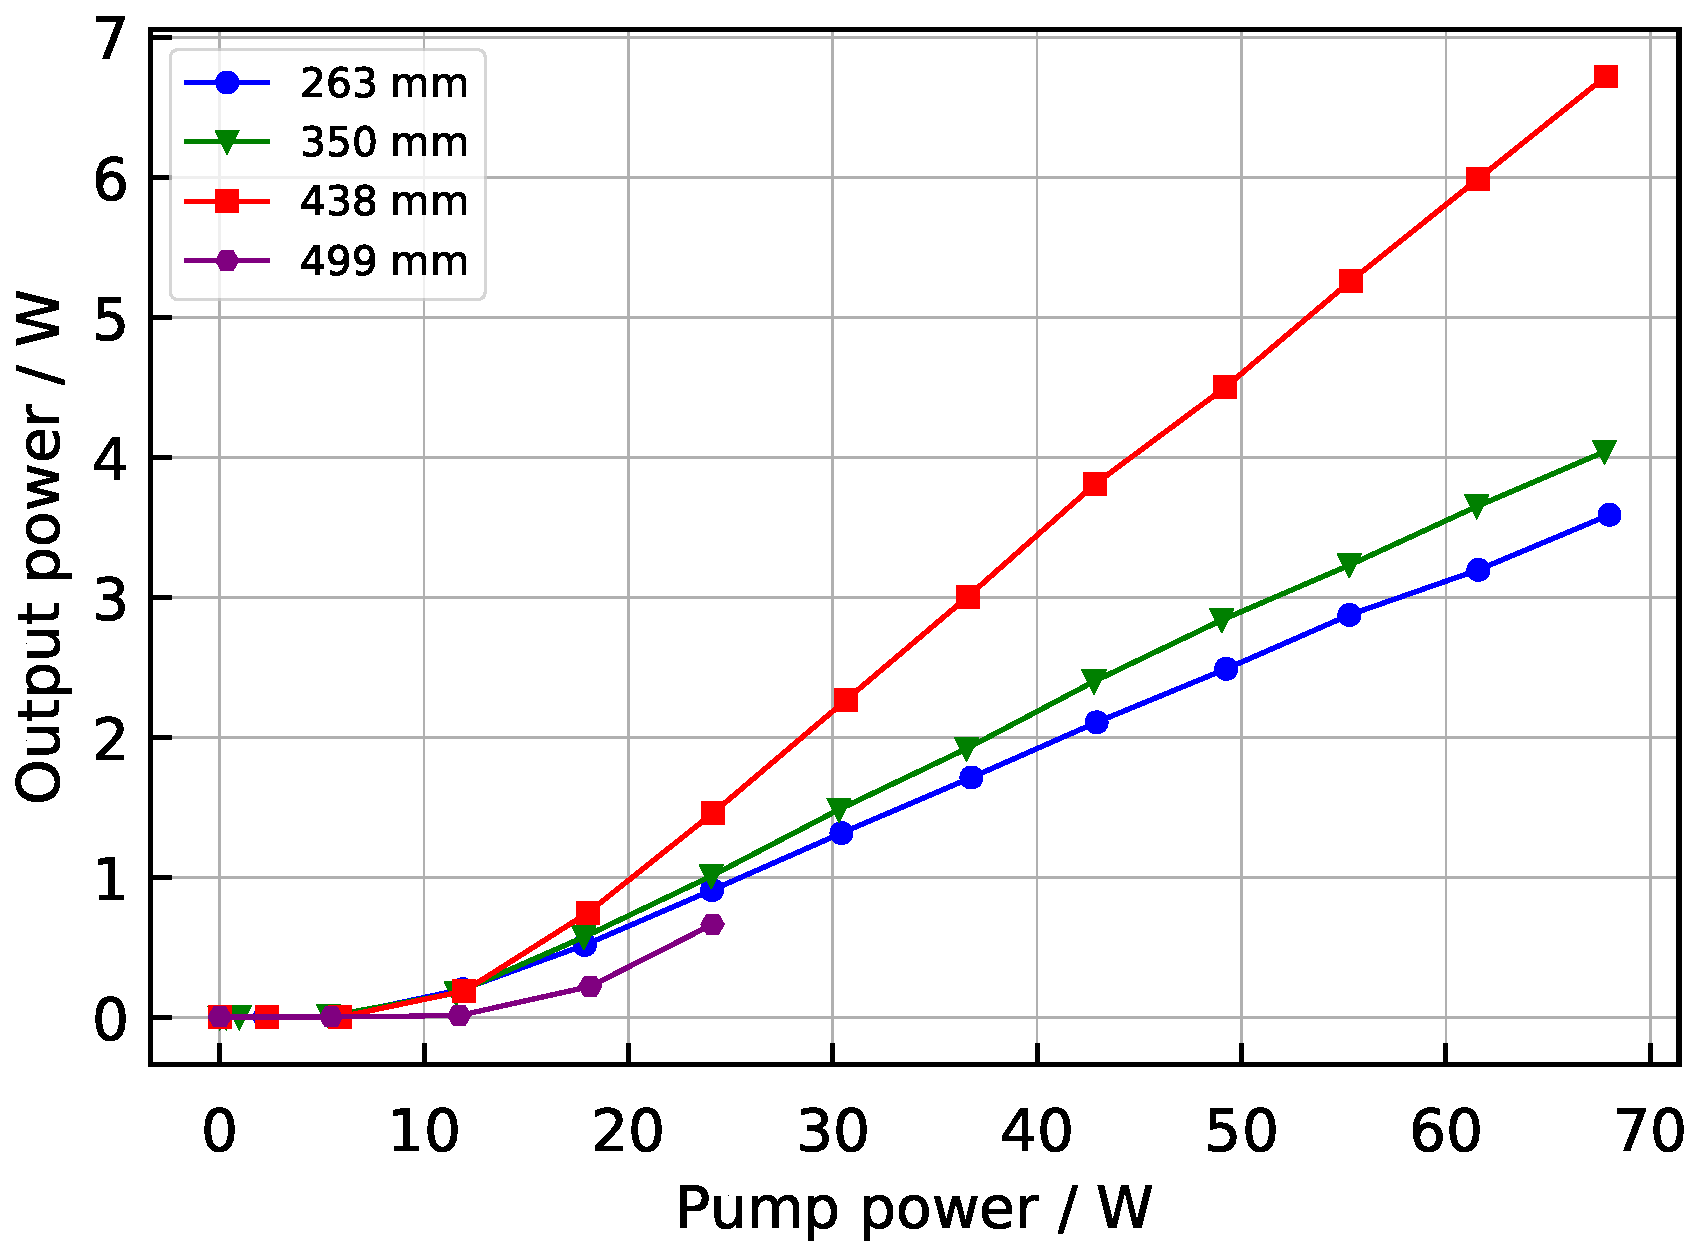
\includegraphics[keepaspectratio, width=0.9\linewidth]{./Figure/Yb1200-20-125DC-PM_SignalComparisonByLength_915Pump976Seed_Exp}
    \subcaption{}
  \end{minipage}
  \begin{minipage}[b]{0.5\linewidth}
    \centering
    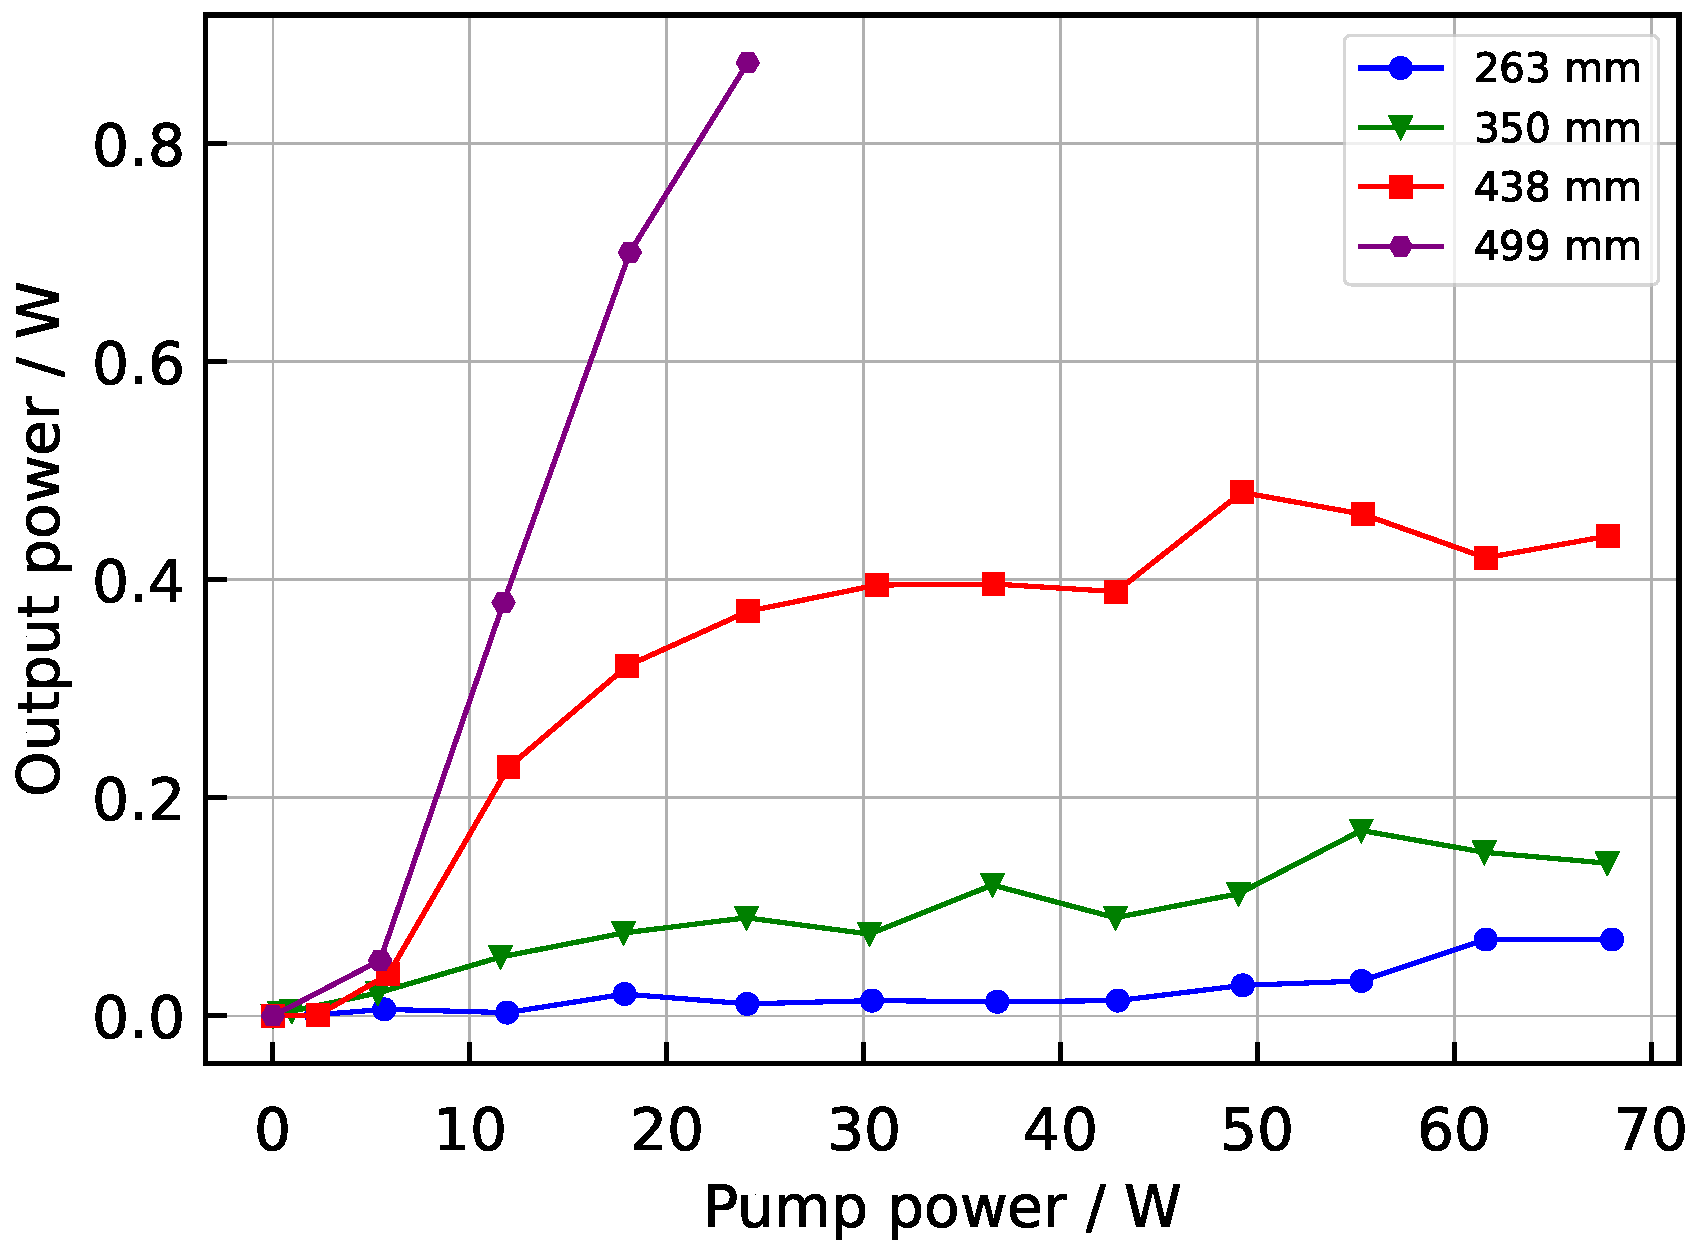
\includegraphics[keepaspectratio, width=0.9\linewidth]{./Figure/Yb1200-20-125DC-PM_ASEComparisonByLength_915Pump976Seed_Exp}
    \subcaption{}
  \end{minipage}
  \caption{Measured \SI{976}{nm} and ASE around \SI{1030}{nm} power as a function of the launched \SI{915}{nm} pump power.}
  \label{fig:OutputComparisonOfNLIGHT976YDFA}
\end{figure}

We measured the output of YDFAs with the \SI{263}{mm}, \SI{350}{mm}, \SI{438}{mm}, and \SI{499}{mm} length of Yb-doped fibers at pump powers up to about \SI{70}{W}.
The output powers are shown in Fig.~\ref{fig:OutputComparisonOfNLIGHT976YDFA}.
As increasing the length of Yb-doped fiber, the \SI{976}{nm} output power increases, reaching maximum at length of \SI{438}{mm}.
For the \SI{438}{mm} fiber, the gain of \SI{976}{nm} began to exceed 1 at the pump power of \SI{12}{W}, and \SI{6.7}{W} output of \SI{976}{nm} was achieved with a slope efficiency of 0.12.
The maximum \SI{976}{nm} gain corresponds to \SI{14.5}{dB}.
In the test of \SI{976}{nmm} fiber, we applied the pump power less than \SI{25}{W} because the ASE power significantly increased.

\begin{figure}[h!]
  \centering
  \begin{minipage}[b]{0.5\linewidth}
    \centering
    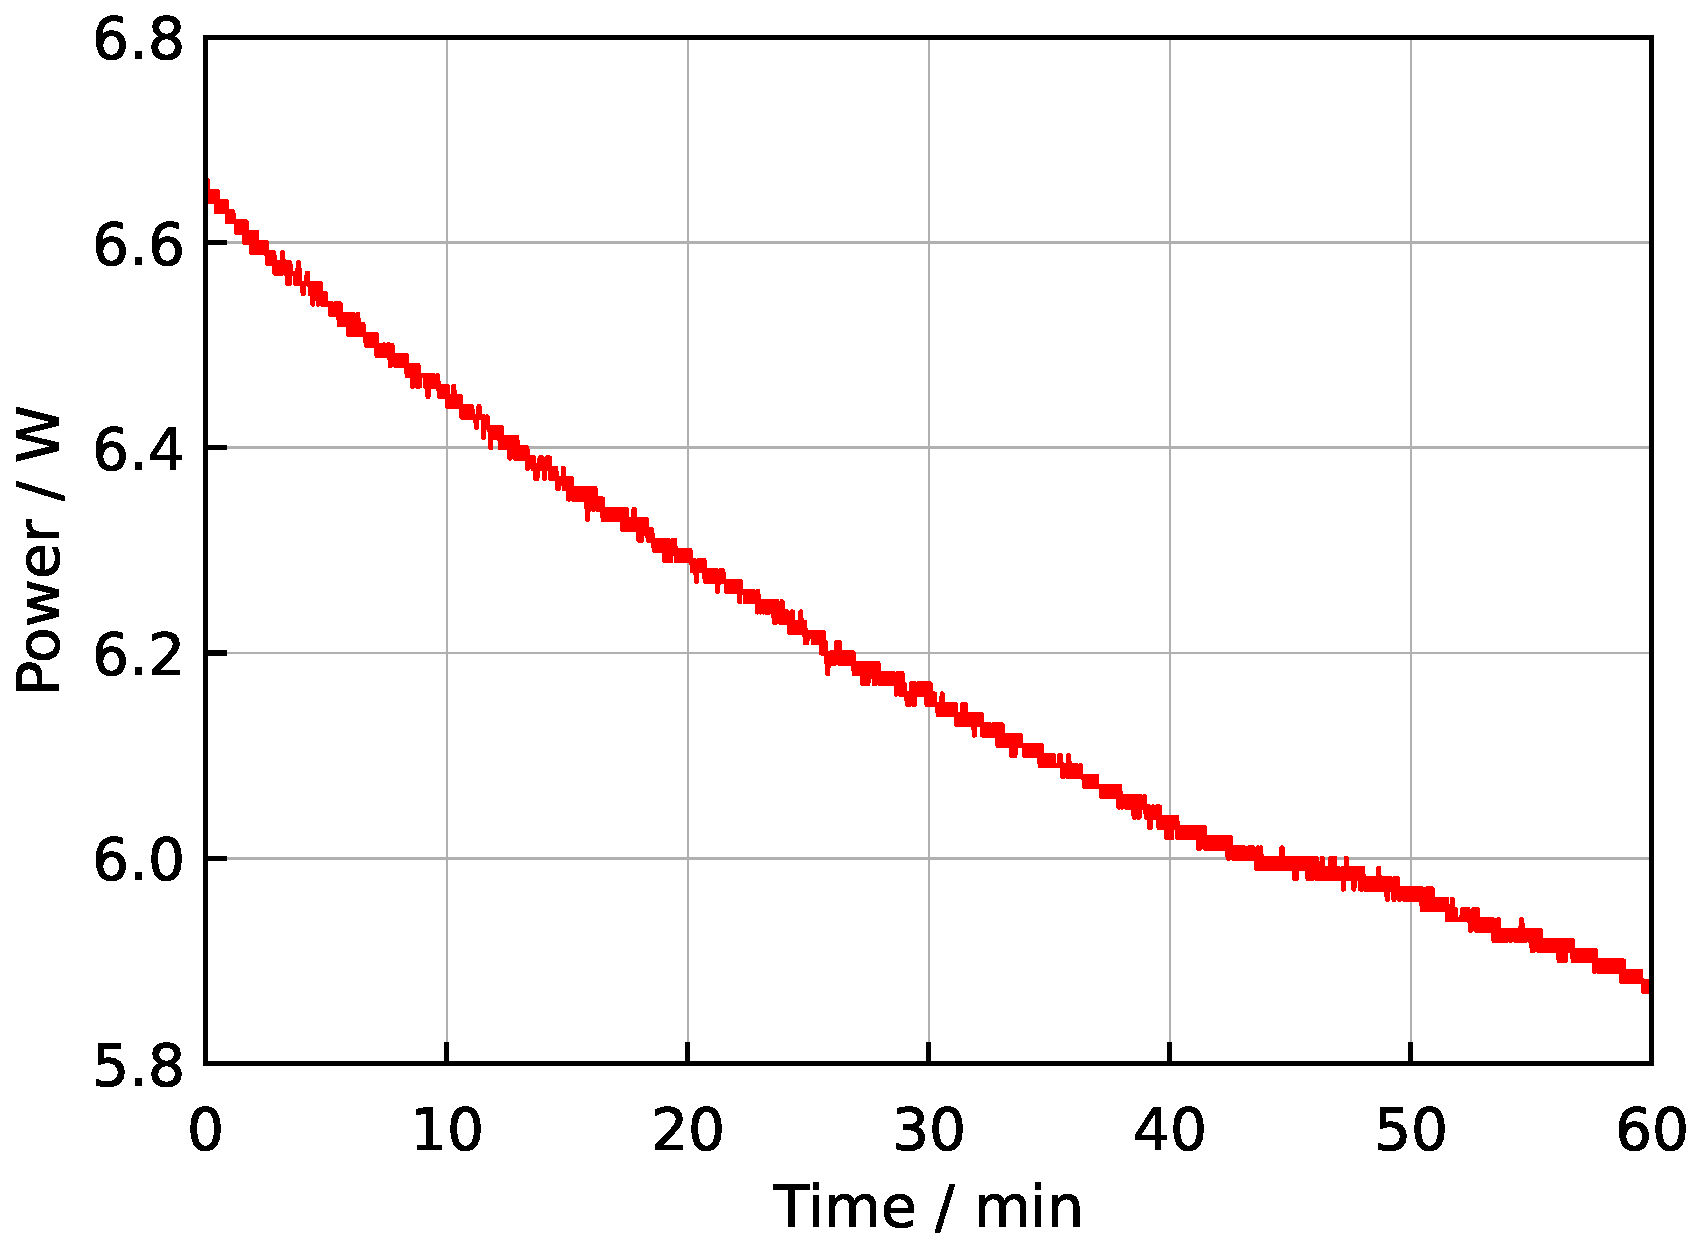
\includegraphics[keepaspectratio, width=0.9\linewidth]{./Figure/Yb1200-20-125DC-PM438mm_LongTermStability_915Pump70W976Seed0.24W_Exp}
    % \subcaption{}
  \end{minipage}
  \caption{Measured output power of the \SI{976}{nm} fiber amplifier as a function of the launched \SI{915}{nm} pump power and results of the simulation.}
  \label{fig:LongTermStabilityOfNLIGHT976YDFA}
\end{figure}

Figure~\ref{fig:LongTermStabilityOfNLIGHT976YDFA} shows \SI{976}{nm} output stability of the \SI{438}{mm} Yb-doped fiber.
The output decays in time to decrease by about 12\% of its original power after \SI{60}{\minute}.
This is mainly due to photodarkening caused by the high-inversion distribution of Yb ion \cite{paschottaLifetimeQuenchingYbdoped1997}.
To avoid power decay by photodarkening, we tested Yb-doped phosphosilicate fiber(Coractive, DCF-YB-20/128P-FAC).
We measured the output of the Yb-doped fiber by changing the fiber length, and obtained the results shown in the Fig.~\ref{fig:OutputComparisonOfCORACTIVE976YDFA}.
The \SI{976}{nm} output power reached a maximum of \SI{5.3}{W} at the \SI{172}{mm} length fiber.

\begin{figure}[h!]
  \begin{minipage}[b]{0.5\linewidth}
    \centering
    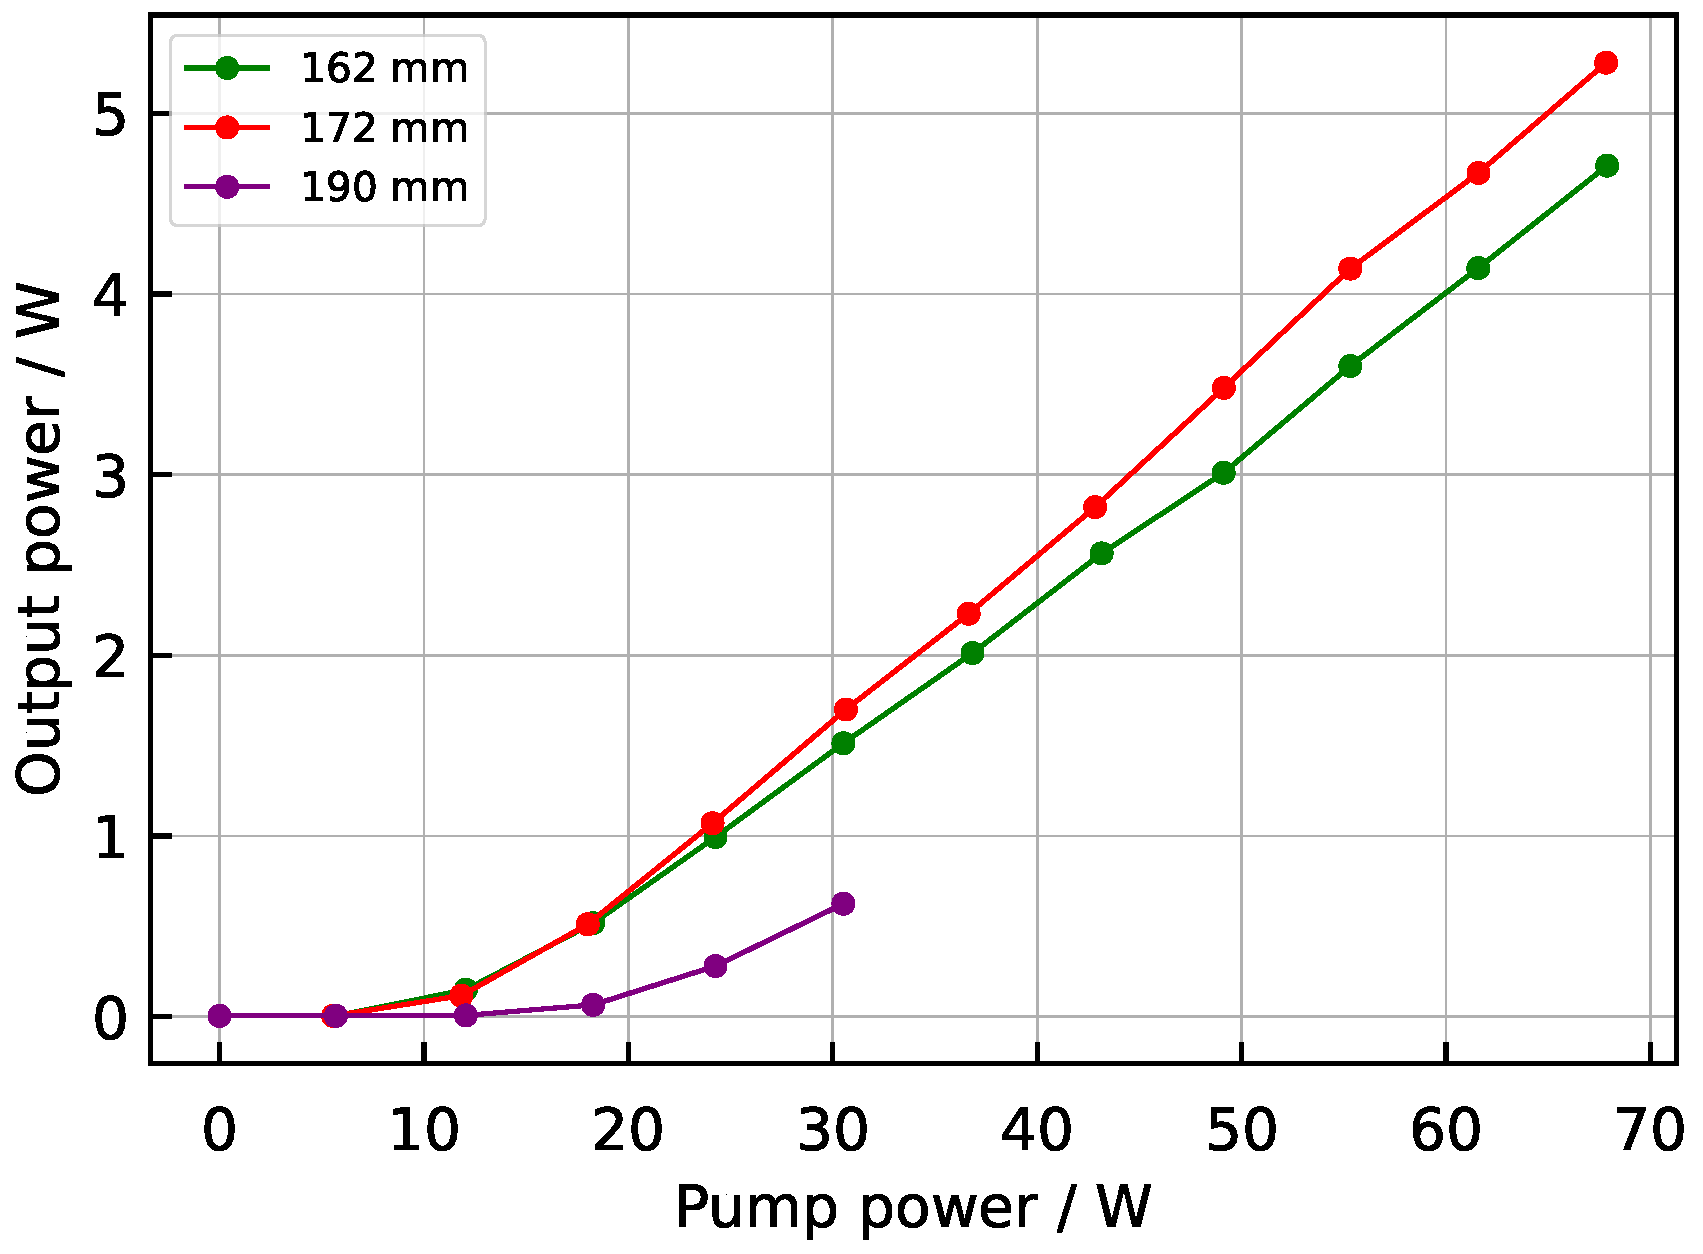
\includegraphics[keepaspectratio, width=0.9\linewidth]{./Figure/DCF-YB-20-128P-FAC172mm_SignalComparisonByLength_915Pump976Seed0.24W_Exp}
    \subcaption{}
  \end{minipage}
  \begin{minipage}[b]{0.5\linewidth}
    \centering
    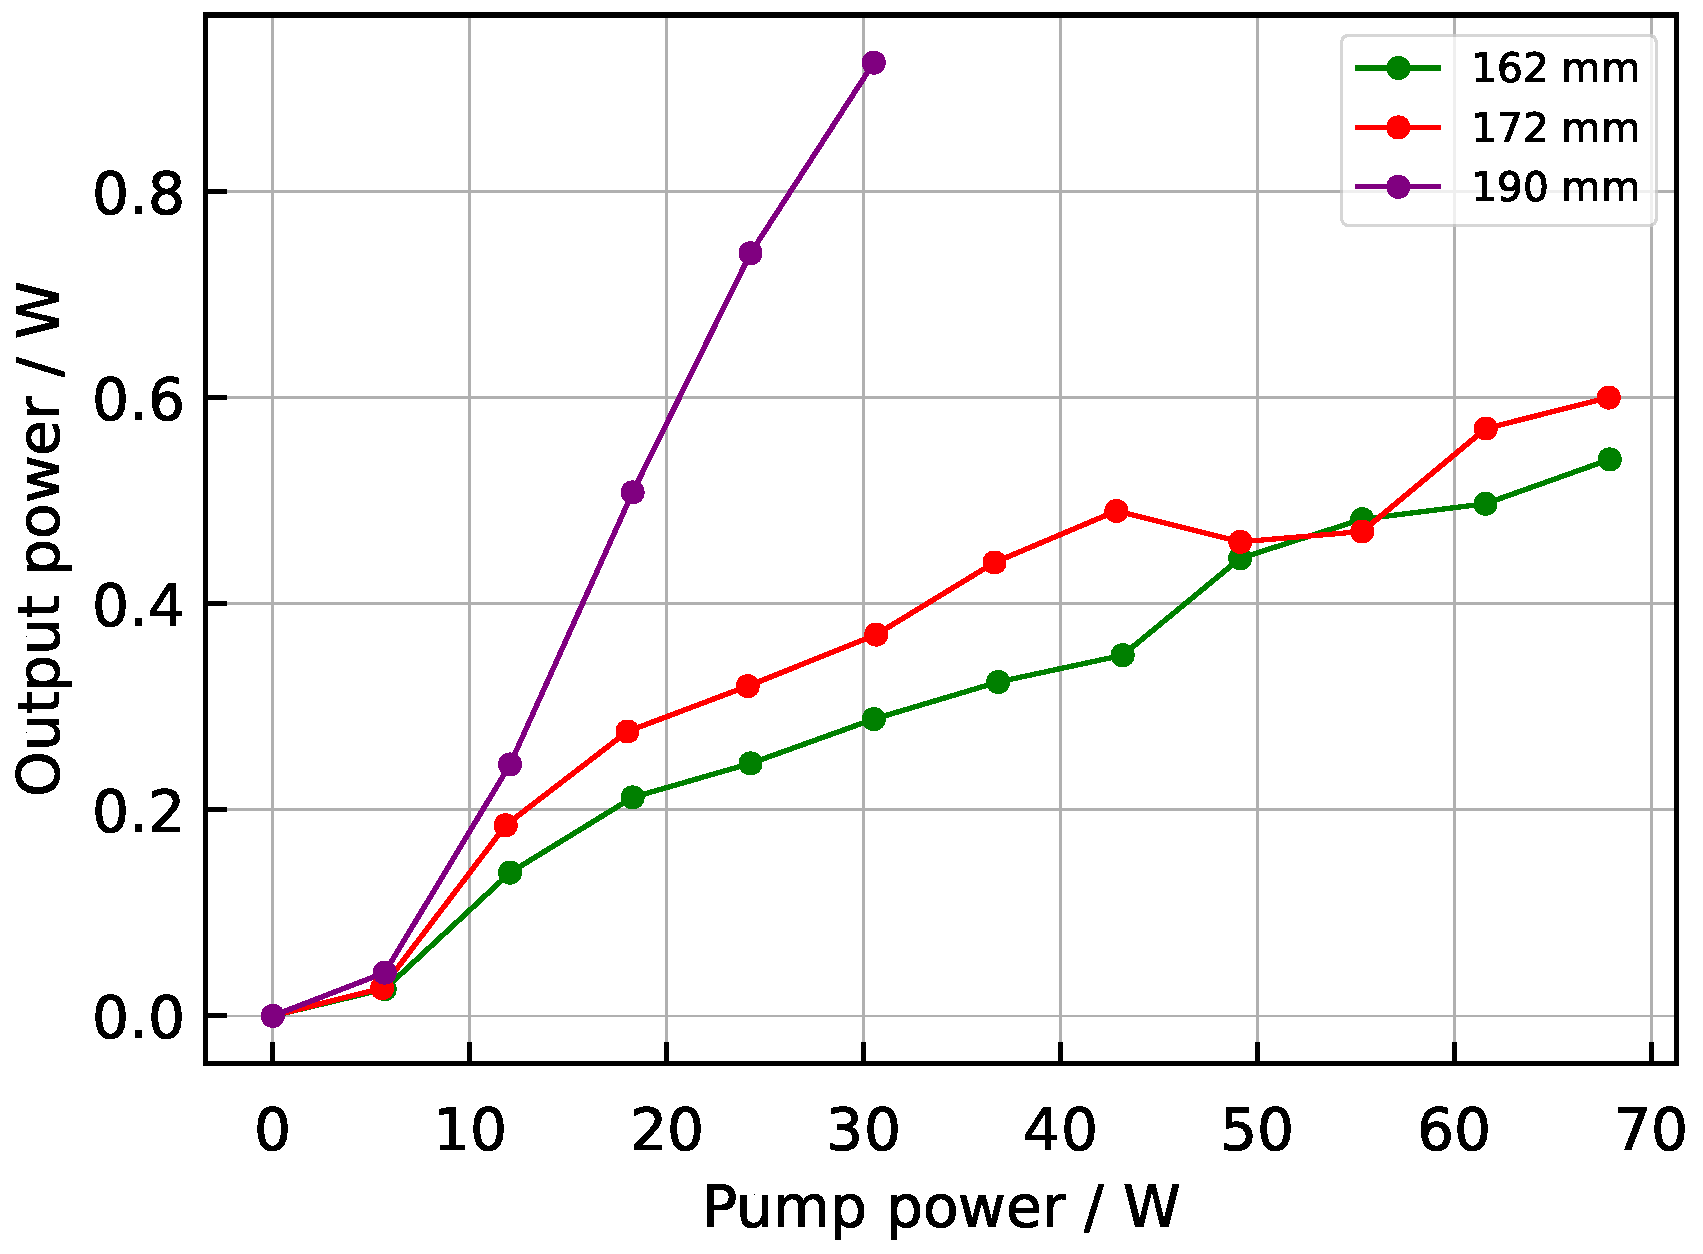
\includegraphics[keepaspectratio, width=0.9\linewidth]{./Figure/DCF-YB-20-128P-FAC172mm_ASEComparisonByLength_915Pump976Seed0.24W_Exp}
    \subcaption{}
  \end{minipage}
  \caption{Measured \SI{976}{nm} and ASE around \SI{1030}{nm} power as a function of the launched \SI{915}{nm} pump power.}
  \label{fig:OutputComparisonOfCORACTIVE976YDFA}
\end{figure}


\begin{figure}[h!]
  \centering
  \begin{minipage}[b]{0.5\linewidth}
    \centering
    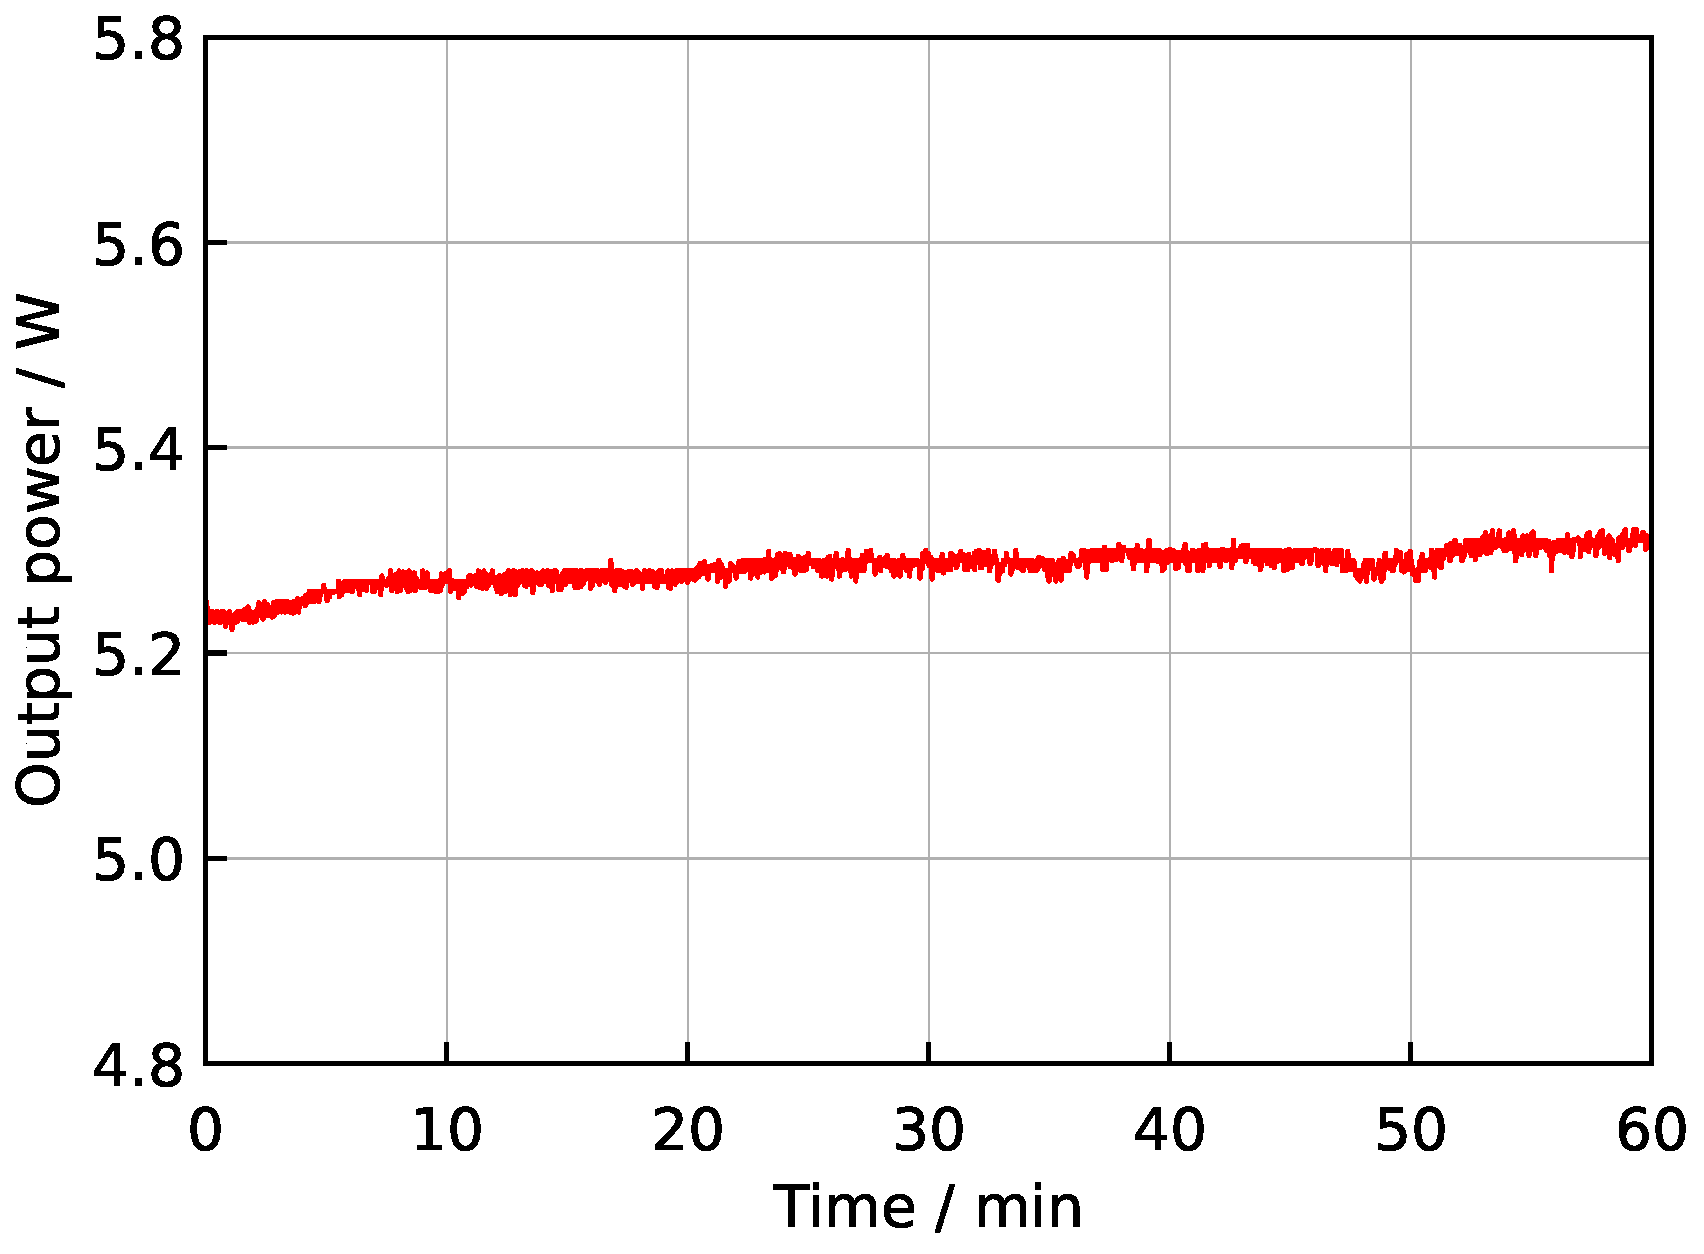
\includegraphics[keepaspectratio, width=0.9\linewidth]{./Figure/DCF-YB-20-128P-FAC172mm_SignalLongTermStability_915Pump70W976Seed0.24W_Exp}
    %\subcaption{}
  \end{minipage}
  \caption{Measured output power of the \SI{976}{nm} fiber amplifier as a function of the launched \SI{915}{nm} pump power and results of the simulation.}
  \label{fig:LongTermStabilityOfCORACTIVE976YDFA}
\end{figure}


\subsection{1112\,nm YDFA}


\section{Discussion}

\section{Conclusion}
\begin{comment}
  The Universal Manuscript Template is based on the Express journal layout and will provide an accurate length estimate for \emph{Optics Express}, \emph{Biomedical Optics Express},  \emph{Optical Materials Express}, and our newest title \emph{OSA Continuum}
  \emph{Applied Optics}, JOSAA, JOSAB, \emph{Optics Letters}, \emph{Optica}, and \emph{Photonics Research} publish articles in a two-column layout
  To estimate the final page count in a two-column layout, multiply the manuscript page count (in increments of 1/4 page) by 60\%
  For example, 11.5 pages in the Universal Manuscript Template are roughly equivalent to 7 composed two-column pages
  Note that the estimate is only an approximation, as treatment of figure sizing, equation display, and other aspects can vary greatly across manuscripts
  Authors of Letters may use the legacy template for a more accurate length estimate.
\end{comment}

\begin{backmatter}

\bmsection{Funding}
Content in the funding section will be generated entirely from details submitted to Prism
Authors may add placeholder text in the manuscript to assess length, but any text added to this section in the manuscript will be replaced during production and will display official funder names along with any grant numbers provided
If additional details about a funder are required, they may be added to the Acknowledgments, even if this duplicates information in the funding section
See the example below in Acknowledgements.

\bmsection{Acknowledgments}
Acknowledgments should be included at the end of the document
The section title should not follow the numbering scheme of the body of the paper
Additional information crediting individuals who contributed to the work being reported, clarifying who received funding from a particular source, or other information that does not fit the criteria for the funding block may also be included; for example, ``K. Flockhart thanks the National Science Foundation for help identifying collaborators for this work.''

\end{backmatter}

%%%%%%%%%%%%%%%%%%%%%%% References %%%%%%%%%%%%%%%%%%%%%%%%%

%%%%%%%%%% If using BibTeX:
\bibliography{2022YDFA}

%%%%%%%%%% If preparing manually:
% \begin{thebibliography}{1}
% \newcommand{\enquote}[1]{``#1''}

% \bibitem{Zhang:14}
% Y.~Zhang, S.~Qiao, L.~Sun, Q.~W. Shi, W.~Huang, L.~Li, and Z.~Yang,
%   \enquote{Photoinduced active terahertz metamaterials with nanostructured
%   vanadium dioxide film deposited by sol-gel method,}
%   {\protect\JournalTitle{Optics Express}} \textbf{22}, 11070--11078 (2014).

% \bibitem{OSA}
% {Optical Society}, \enquote{{OSA Publishing},}
%   \url{http://www.osapublishing.org}.

% \bibitem{FORSTER2007}
% P.~Forster, V.~Ramaswamy, P.~Artaxo, T.~Bernsten, R.~Betts, D.~Fahey,
%   J.~Haywood, J.~Lean, D.~Lowe, G.~Myhre, J.~Nganga, R.~Prinn, G.~Raga,
%   M.~Schulz, and R.~V. Dorland, \enquote{Changes in atmospheric consituents and
%   in radiative forcing,} in \enquote{Climate Change 2007: The Physical Science
%   Basis. Contribution of Working Group 1 to the Fourth assesment report of
%   Intergovernmental Panel on Climate Change,}  S.~Solomon, D.~Qin, M.~Manning,
%   Z.~Chen, M.~Marquis, K.~B. Averyt, M.~Tignor, and H.~L. Miler, eds.
%   (Cambridge University Press, 2007).

% \end{thebibliography}

\end{document}
